\chapter{Sampling, optimisation and cosmology fitting}\label{ch:sampling-fitting}
\chapterstatus{written}{2026-11-19}

General samplers and optimisers for any posterior (adaptive Metropolis--Hastings, Hamiltonian Monte Carlo, Nelder--Mead with profile
likelihoods), convergence diagnostics, and the program \file{./mcmc} that fits cosmological parameters to supernova, BAO and CMB data with
the Einstein--Boltzmann solver as the theory.

\begin{modulebox}{MCMC, CosmologyFitting}
\nsp{FML::MCMC}: \file{MCMC/Posterior.h} (\cls{Posterior}, \cls{SampledParameter}), \file{MCMC/Sampler.h} (\cls{Sampler}), \file{MCMC/Minimizer.h}
(\cls{Minimizer}), \file{MCMC/HMC.h} (\code{run_hmc}, \cls{HMCOptions}, \cls{HMCMass}), \file{MCMC/HMCCheckpoint.h}, \file{MCMC/Diagnostics.h}
(\code{diagnose_chains}), \file{MCMC/Parallel.h}. \nsp{FML::COSMOLOGY::FITTING}: \file{CosmologyFitting/Theory.h}, \file{Likelihoods.h},
\file{SampledParameterMap.h}; the program \file{CosmologyFitting/mcmc} with parameter files in \file{params/} and data in \file{external/}.\par
Documentation: \file{MCMC/README.md}, \file{CosmologyFitting/README.md}. Tests: \file{MCMC/tests}, \file{CosmologyFitting/tests}.
\end{modulebox}

\section{Metropolis--Hastings}\label{sec:fit-mh}

\cls{Sampler} runs several chains in parallel (OpenMP threads and MPI processes) for a \cls{Posterior}: sampled parameters with flat priors, optional
Gaussian priors and a proposal step, derived parameters, and a likelihood function. During burn-in the proposal covariance and scale adapt towards 25\%
acceptance \cite{Haario2001}; at the end of burn-in the covariance pooled from all chains is frozen, so the sampling phase is an exact Markov chain. Points
where the likelihood throws or is not finite are rejected. Fast parameters (e.g.\ likelihood nuisances, for which the theory is cached) get extra updates along
their conditional covariance \cite{Lewis2013}. The run stops when every chain has enough samples and the multivariate Gelman--Rubin $R-1$ (the largest eigenvalue
of $W^{-1}B$, as CosmoMC and Cobaya \cite{Gelman1992}) is below the threshold. Checkpoints hold the complete chain state, so a resumed run continues exactly as
an uninterrupted one, with any number of processes. Output is in GetDist format.

\section{Hamiltonian Monte Carlo}\label{sec:fit-hmc}

\file{HMC.h} samples a potential $U=-\ln p$ with its gradient \cite{Duane1987,Neal2011}, for problems with many parameters such as field-level inference
(\cref{ch:field-level}). The state is a custom block (e.g.\ a field) with a mass given as operators ($M^{1/2}$ on white noise and $M^{-1}$; nothing of it is
recorded) followed by parameters with a diagonal mass adapted in Stan's windows. Leapfrog with a jittered number of steps; the step size is adapted by dual
averaging \cite{HoffmanGelman2014} to a target acceptance; bounds are handled by reflection; divergences are counted. \cls{HMCState} holds the complete state
(including the random generator and adaptation) for exact continuation, with a versioned, checksummed binary codec.

\section{Optimisation and profiles}\label{sec:fit-minimizer}

\cls{Minimizer} maximises the posterior with the Nelder--Mead simplex with adaptive coefficients \cite{GaoHan2012} in coordinates whitened by a covariance,
restarting around the best point until a restart gains less than a tolerance, from several starts in parallel; with fast parameters an inner simplex minimises
them at each slow point. \code{profile} gives profile likelihoods (independent of priors and volume effects) and \code{hessian} the covariance from central
differences with adapted steps.

\section{Diagnostics}\label{sec:fit-diagnostics}

\file{Diagnostics.h} implements the rank-normalised split-$\hat R$, its folded version, and bulk and tail effective sample sizes \cite{Vehtari2021}: ranks with
average ties and Blom scores $(r-3/8)/(S+1/4)$, multi-chain variance, FFT autocovariances and Geyer's initial positive/monotone sequence; the tail ESS is the
minimum of the 5\% and 95\% quantile-indicator ESS. Degenerate cases (too few chains or draws, frozen chains, non-finite values) are reported as statuses rather
than numbers. $\hat R<1.01$ and ESS above $\sim100$ per chain are screening criteria, not guarantees.

\begin{validation}[Validation: samplers]
Sampler: correlated Gaussians, priors, rejected regions, GetDist output, fast/slow and checkpoint/resume. HMC: diagonal mass adaptation over six decades of
variance, an operator mass block coupled to parameters, reflection at bounds. Minimiser: a 4D Gaussian with a prior (maximum to $<0.005\sigma$), Rosenbrock
($2\times10^{-5}$), a maximum on a prior boundary, two peaks, fast/slow, exact profile and Hessian covariance. Diagnostics: fixtures from ArviZ 0.21.0.
\end{validation}

\section{Cosmology fitting}\label{sec:fit-cosmology}

\file{./mcmc} reads a parameter file in the format of the solver's \file{./cmb} (\cref{ch:background}): any solver parameter can be fixed, \code{sample_<name> =
start, min, max, step} samples it (also the aliases \code{H0}, \code{omega_b}, \code{omega_cdm}, \code{Omega_m}, \code{logA}, \code{tau_reio} and
\code{theta_MC_100}), and \code{sampler} selects \code{mcmc}, \code{minimize} (with profiles and a Hessian) or \code{hessian}. The theory is computed only as far as
the likelihoods need: the background for supernovae; the recombination history for BAO and distance priors ($r_d$, $z_*$); the full lensed CMB spectra for the
CMB likelihoods. The likelihoods:
\begin{itemize}
\item supernovae: Pantheon+ \cite{Brout2022}, DES-SN5YR \cite{DESY5}, DES-Dovekie \cite{Popovic2025} and Union3 \cite{Rubin2023}, with the absolute magnitude
      marginalised analytically;
\item BAO: DESI DR1 and DR2 with full covariance \cite{DESI2025}; BBN $\omega_b$;
\item DESI DR1 full shape \cite{DESI2024VII}: the rotated $P_0$, $P_2$ of the six samples with their window and systematics, as DESI's own likelihood: velocileptors'
      REPT with the loops of the linear $P_{cb}$ at the first redshift scaled by $D^4$, the linear terms and $f(k)=(P_{\theta\theta}/P_{cb})^{1/2}$ at each redshift
      (\cref{ch:perturbation-theory}), the peak-average no-wiggle filter, AP, the physical bias basis and the counterterms and stochastic terms marginalised analytically;
\item CMB: Planck 2018 distance priors \cite{Chen2019DP}, plik\_lite TTTEEE/TT with the low-$\ell$ TT compressed \cite{Planck2018spectra,PrinceDunkley2019}, the Planck 2018
      lensing likelihood \cite{Planck2018lensing} (also CMB-marginalised), Planck 2018's low-$\ell$ TT (Commander) and EE (SimAll) likelihoods
      \cite{Planck2018spectra} and the high-$\ell$ CamSpec PR4 (NPIPE) TTTEEE likelihood \cite{Rosenberg2022} with its foreground residuals and calibrations (ported from
      Cobaya), the ACT DR6 (+ Planck PR4) lensing likelihood \cite{Madhavacheril2023,Qu2023} with its CMB-dependent normalisation and $N_1$ corrections
      (linear in the spectra, precomputed as matrices on the bandpowers), and an exact mock Gaussian likelihood of TT, TE, EE (and BB) for forecasts and tests.
\end{itemize}
With several likelihoods each $\chi^2$ is a derived parameter, as are $H_0$, $\Om$, the age, $r_d$, $\theta_*$, $\sigma_8$ and $S_8$.

\paragraph*{The Fading Dark Sector.} \file{params/mcmc_fds_cmb_desi_dovekie.ini} and \file{mcmc_fds_cmb_desi15_dovekie.ini} are the fits
of Obied, Vafa \& Wu \cite{ObiedVafaWu2026} (\code{model = fading_dark_sector}, $c$ and $c'\ge0$ sampled): CamSpec PR4, the Planck low-$\ell$ TT
and EE, ACT DR6 + Planck PR4 lensing, DESI DR2 BAO and DES-Dovekie, with the DESI DR1 full shape in the second. The nonlinear lensing and shear
spectra can use \code{nonlinear = react}, which supports the coupled dark matter (\cref{sec:hm-react}). The full shape uses EdS loop kernels
with the model's linear $P_{cb}$, $P_{\theta\theta}$ and growth, whereas the paper uses exact-time two-fluid kernels (CDM with the fifth force
and the drag, baryons without). \file{tests/check_fds_kernels} computes both for the same linear $P_{cb}$: at $c=-0.85$, $c'=0.053$,
$z=0.3$--1.5 and $k\le0.2\hMpc$ the exact-time $\delta\delta$ loop differs from EdS by $\le3\times10^{-3}$ of $P_L$ and the $\theta\theta$
loop by $\le1\%$ of $f^2P_L$, almost all of it present in $\Lambda$CDM as well; the part due to the fifth force and the drag is
$\le4\times10^{-4}$ and $3\times10^{-3}$. Mapped onto the DESI multipoles (\file{python/fds_kernels_dchi2.py}) the whole difference
changes $\chi^2$ by 0.011 (0.001 after refitting $b_1$, $\alpha_0$, $\alpha_2$ and the shot noise) and the FDS-specific part by 0.001,
against the model's $\Delta\chi^2\approx-14$ to $-20$: EdS kernels are enough for these fits.

\begin{paramfile}[A w0wa fit to DESI DR2, Planck distance priors and Pantheon+]
model       = w0wa
likelihoods = desi_dr2, planck_dp, pantheonplus
sample_H0      = 68, 50, 90, 0.5, H_0
sample_omega_b = 0.0224, 0.019, 0.026, 0.0002, \omega_b
sample_Omega_m = 0.31, 0.2, 0.4, 0.005, \Omega_m
sample_w0      = -0.9, -2, 0, 0.05, w_0
sample_wa      = -0.5, -3, 2, 0.2, w_a
mcmc_chains = 4
mcmc_output = chains/w0wa
\end{paramfile}

\begin{validation}[Validation: cosmology fitting]
Distances against independent integrals, $r_d$ against CLASS to $10^{-4}$, the distance priors at the Planck best fit within $0.3\sigma$; plik\_lite equal to planck-lite-py
to $10^{-13}$ in $\ln L$ and the lensing likelihood equal to Cobaya's to $10^{-14}$; supernova likelihoods equal to an independent Python implementation to $10^{-5}$ in
$\chi^2$; the Planck low-$\ell$ TT and EE likelihoods equal to Cobaya's to $10^{-14}$ in $\ln L$ and CamSpec PR4 to $10^{-8}$ (relative) in $\chi^2$, ACT DR6 lensing equal to act\_dr6\_lenslike to $10^{-14}$; DESI DR1 full shape equal to DESI's code path (velocileptors) to $10^{-7}$ in $\ln L$ for the same
linear inputs, whose $P_{cb}$ agrees with CAMB's to $10^{-4}$. DESI DR2 + BBN gives $\Om=0.2975\pm0.0085$, $hr_d=101.53\pm0.72$\,Mpc, $H_0=68.53\pm0.60$, as the DESI analysis. DESI DR2 + distance priors + Pantheon+ in $w_0w_a$:
$w_0=-0.848\pm0.054$, $w_a=-0.55\pm0.22$, $\Delta\chi^2=-7.6$ against $\Lambda$CDM. The plik\_lite (+ lensing) best fit agrees with the Planck 2018 best-fit parameters to a
fraction of $\sigma$; mock CMB fits with isocurvature, tensors or ultralight axions recover the fiducial values.
\end{validation}

\begin{figure}[htbp]
\centering
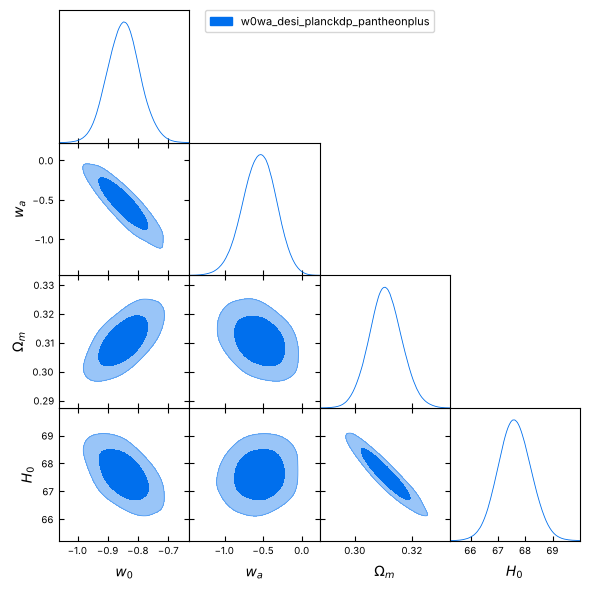
\includegraphics[width=0.6\textwidth]{fitting_w0wa}
\caption{Marginalised posteriors of $w_0$, $w_a$, $\Om$ and $H_0$ from DESI DR2 BAO, the Planck 2018 distance priors and Pantheon+ with
\file{./mcmc} (\file{params/mcmc_w0wa.ini}; 68\% and 95\% contours).}
\label{fig:fit-w0wa}
\end{figure}

